\documentclass{article}
\usepackage{import}
\subimport*{./}{macro}

\setlength\parindent{0px}

\begin{document}
\setcounter{aprob}{0}
\setcounter{bprob}{0}
\title{Homework \#0}
\author{
    \normalsize{CSE 446/546: Machine Learning}\\
    \normalsize{Profs. Jamie Morgenstern and Simon Du}\\
    \normalsize{Due: \textbf{Wednesday} October 6, 2021 11:59pm}\\
    \normalsize{\textbf{A:} 38 points, \textbf{B:} 7 points}
}
\date{{}}
\maketitle

\noindent Please review all homework guidance posted on the website before submitting to GradeScope. Reminders:
\begin{itemize}
    \item Make sure to read the ``What to Submit'' section following each question and include all items.
    \item Please provide succinct answers and supporting reasoning for each question. Similarly, when discussing experimental results, concisely create tables and/or figures when appropriate to organize the experimental results. All explanations, tables, and figures for any particular part of a question must be grouped together.
    \item For every problem involving generating plots, please include the plots as part of your PDF submission.
    \item When submitting to Gradescope, please link each question from the homework in Gradescope to the location of its answer in your homework PDF. Failure to do so may result in deductions of up to \points{5}. For instructions, see \url{https://www.gradescope.com/get_started#student-submission}.
    \item Please recall that B problems, indicated in \boxed{\textrm{boxed text}}, are only graded for 546 students, and that they will be weighted at most 0.2 of your final GPA (see website for details). In Gradescope there is a place to submit solutions to A and B problems separately. You are welcome to create just a single PDF that contains answers to both, submit the same PDF twice, but associate the answers with the individual questions in Gradescope. 
    \item If you collaborate on this homework with others, you must indicate who you worked with on your homework. Failure to do so may result in accusations of plagiarism.
    \item For every problem involving code, please include the code as part of your PDF for the PDF submission \emph{in addition to} submitting your code to the separate assignment on Gradescope created for code. Not submitting all code files will lead to a deduction of \points{1}.  
\end{itemize}

Not adhering to these reminders may result in point deductions. \\

% \textcolor{red}{\textbf{Changelog:}}

% \begin{itemize}
%     \item \textbf{Date:} Changed This.
% \end{itemize}

\clearpage{}


% Start of Problems:

\section*{Probability and Statistics}
\begin{aprob}
    \points{2} (From Murphy Exercise 2.4.) 
    After your yearly checkup, the doctor has bad news and good news. 
    The bad news is that you tested positive for a serious disease, and that the test is 99\% accurate (i.e., the probability of testing positive given that you have the disease is 0.99, as is the probability of testing negative given that you don't have the disease).
    The good news is that this is a rare disease, striking only one in 10,000 people.
    What are the chances that you actually have the disease?
    
    \subsubsection*{What to Submit:}
    \begin{itemize}
        \item Final Answer
        \item Corresponding Calculations
    \end{itemize}
\end{aprob}

\begin{aprob}
    For any two random variables $X,Y$ the \emph{covariance} is defined as $\Cov{X}{Y}=\E{(X-\E{X})(Y-\E{Y})}$. 
    You may assume $X$ and $Y$ take on a discrete values if you find that is easier to work with.
    \begin{enumerate}
        \item \points{1} If $\E{Y\given X=x} = x$ show that $\Cov{X}{Y} = \E{\round{X-\E{X}}^2}$.  
        \item \points{1} If $X, Y$ are independent show that $\Cov{X}{Y}=0$.
    \end{enumerate}

    \subsubsection*{What to Submit:}
    \begin{itemize}
        \item \textbf{Parts a-b:} Proofs
    \end{itemize}
\end{aprob}

\begin{aprob}
    Let $X$ and $Y$ be independent random variables with PDFs given by $f$ and $g$, respectively.
    Let $h$ be the PDF of the random variable $Z = X+Y$.
    \begin{enumerate}
        \item \points{1} Show that $h(z) = \int_{-\infty}^\infty f(x) g( z - x ) \diff x $.  (If you are more comfortable with discrete probabilities, you can instead derive an analogous expression for the discrete case,  and then you should give a one sentence explanation as to why your expression is analogous to the continuous case.).
        \item \points{1} If $X$ and $Y$ are both independent and uniformly distributed on $[0,1]$ (i.e. $f(x)=g(x)=1$ for $x \in [0,1]$ and $0$ otherwise) what is $h$, the PDF of $Z=X+Y$?
    \end{enumerate}

    \subsubsection*{What to Submit:}
    \begin{itemize}
        \item \textbf{Part a:} Proof
        \item \textbf{Part b:} Formula for PDF $Z$ and corresponding calculations
    \end{itemize}
\end{aprob}

\begin{aprob}
    Let $X_1, X_2, ..., X_n \sim \mathcal{N}(\mu, \sigma^2)$ be i.i.d random variables. Compute the following:
    \begin{enumerate}
        \item \points{1} $a,b$ such that $aX_1+b \sim \mathcal{N}(0,1)$.
        \item \points{1} $\E{X_1 + 2X_2}, \Var{X_1 + 2X_2}$.
        \item \points{2} Setting $\widehat{\mu}_n = \frac{1}{n} \sum_{i=1}^n X_i$, the mean and variance of $\sqrt{n}(\widehat{\mu}_n - \mu)$.
    \end{enumerate}

    \subsubsection*{What to Submit:}
    \begin{itemize}
        \item \textbf{Part a:} $a$, $b$, and the corresponding calculations
        \item \textbf{Part b:} $\E{X_1 + 2X_2}$, $\Var{X_1 + 2X_2}$
        \item \textbf{Part c:} $\E{\sqrt{n}(\widehat{\mu}_n - \mu)}$, $\Var{\sqrt{n}(\widehat{\mu}_n - \mu)}$
        \item \textbf{Parts a-c} Corresponding calculations
    \end{itemize}
\end{aprob}

\begin{bprob}
    \points{1} Let $X_1,\dots,X_n$ be $n$ independent and identically distributed random variables drawn uniformly at random from $[0,1]$. If $Y = \max\set{X_1,\ldots,X_n}$ then find $\E{Y}$.
    \subsubsection*{What to Submit:}
    \begin{itemize}
        \item Expression for $\E{Y}$ and corresponding calculations
    \end{itemize}
\end{bprob}

\begin{bprob}
    \points{1} Let $X$ be random variable with $\E{X} = \mu$ and $\E{(X-\mu)^2} = \sigma^2$. For any $x > 0$, use Markov's inequality to show that $\Prob{ X \geq \mu + \sigma x } \leq 1/x^2$.
    \subsubsection*{What to Submit:}
    \begin{itemize}
        \item Proof
    \end{itemize}
\end{bprob}

\begin{bprob}
    For any function $g \colon \R \to \R$ and random variable $X$ with PDF $f(x)$, recall that the expected value of $g(X)$ is defined as $\E{g(X)} = \int_{-\infty}^\infty g(y) f(y) \diff y$. For a boolean event $A$, define $\1\{ A \}$ as $1$ if $A$ is true, and $0$ otherwise. Fix $F(x) = \E{\1\{X \leq x\}}$. Let $X_1,\ldots,X_n$ be independent and identically distributed random variables with CDF $F(x)$. Define $\widehat{F}_n(x) = \frac{1}{n} \sum_{i=1}^n \1\{X_i \leq x\}$. Note, for every $x$, that $\widehat{F}_n(x)$ is an empirical estimate of  $F(x)$.
    \begin{enumerate}
      \item \points{1} For any $x$, what is $\E{\widehat{F}_n(x)}$?
      \item \points{1} For any $x$, the variance of $\widehat{F}_n(x)$ is $\E{\left( \widehat{F}_n(x) -  F(x) \right)^2 }$.  Show that $\Var{\widehat{F}_n(x)} = \frac{F(x)(1-F(x))}{n}$.
      \item \points{1} Using your answer to b, show that for all $x\in \R$, we have  $\displaystyle \E{ \left( \widehat{F}_n(x) - F(x) \right)^2 } \leq \tfrac{1}{4n}$.  
    \end{enumerate}
    
    \subsubsection*{What to Submit:}
    \begin{itemize}
        \item \textbf{Part a:} Formula for $\E{\widehat{F}_n(x)}$ and corresponding calculations
        \item \textbf{Parts b-c:} Proof
    \end{itemize}
\end{bprob}


\section*{Linear Algebra and Vector Calculus}
\begin{aprob}
    Let $A = \begin{bmatrix} 1 & 2 & 1 \\ 1 & 0 & 3 \\ 1 & 1 & 2 \end{bmatrix}$ and $B = \begin{bmatrix} 1 & 2 & 3 \\ 1 & 0 & 1 \\ 1 & 1 & 2 \end{bmatrix}$.
    For each matrix $A$ and $B$:
    \begin{enumerate} 
    	\item \points{2} What is its rank? 
    	\item \points{2} What is a (minimal size) basis for its column span?
    \end{enumerate}
    
    \subsubsection*{What to Submit:}
    \begin{itemize}
        \item \textbf{Parts a-b:} Solution and corresponding calculations
    \end{itemize}
\end{aprob}

\begin{aprob}\label{prob:linsystem}
    Let $A = \begin{bmatrix} 0 & 2 & 4 \\ 2 & 4 & 2 \\ 3 & 3 & 1 \end{bmatrix}$, $b = \begin{bmatrix} -2 & -2 & -4 \end{bmatrix}^\top$, and $c=\begin{bmatrix} 1 & 1 & 1 \end{bmatrix}^\top$.
    \begin{enumerate}
    	\item \points{1} What is $Ac$?
    	\item \points{2} What is the solution to the linear system $Ax = b$?
    \end{enumerate}
    
    \subsubsection*{What to Submit:}
    \begin{itemize}
        \item \textbf{Parts a-b:} Solution and corresponding calculations
    \end{itemize}
\end{aprob}

\begin{aprob} \label{prob:sumvec}
    For possibly non-symmetric $\mat{A}, \mat{B} \in \R^{n \times n}$ and $c \in \R$, let $f(x, y) = x^\top \mat{A} x + y^\top \mat{B} x + c$. Define
    $$\nabla_z f(x,y) = \begin{bmatrix}
        \pderiv{f}{z_1}(x,y) & \pderiv{f}{z_2}(x,y) & \dots & \pderiv{f}{z_n}(x,y)
    \end{bmatrix}^\top.$$  
    \begin{enumerate}
    	\item \points{2} Explicitly write out the function $f(x, y)$ in terms of the components $A_{i,j}$ and $B_{i,j}$ using appropriate summations over the indices.
    	\item \points{2} What is $\nabla_x f(x,y)$ in terms of the summations over indices \emph{and} vector notation?
    	\item \points{2} What is $\nabla_y f(x,y)$ in terms of the summations over indices \emph{and} vector notation?
    \end{enumerate}
    \subsubsection*{What to Submit:}
    \begin{itemize}
        \item \textbf{Part a:} Explicit formula for $f(x, y)$
        \item{Parts b-c:} Summation form and corresponding calculations
        \item{Parts b-c:} Vector form and corresponding calculations
    \end{itemize}
\end{aprob}

\begin{aprob}\label{prob:matrixtype}
    Show the following:
    \begin{enumerate}
        \item \points{2} Let $g : \R \rightarrow \R$ and $v, w \in \R^n$ such that $g(v_i) = w_i$. Find an expression for $g$ such that $\diag(v)^{-1} = \diag(w)$.
        \item \points{2} Let $\mat{A} \in R^{n \times n}$ be orthonormal and $x \in \R^n$. Show that $||\mat{A}x||_2^2 = ||x||_2^2$.
        \item \points{2} Let $\mat{B} \in R^{n \times n}$ be invertible and symmetric. Show that $\mat{B}^{-1}$ is also symmetric.
        \item \points{2} Let $\mat{C} \in R^{n \times n}$ be positive semi-definite (PSD). Show that its eigenvalues are non-negative.
    \end{enumerate}
    \subsubsection*{What to Submit:}
    \begin{itemize}
        \item \textbf{Part a:} Explicit formula for $g$
        \item \textbf{Parts a-d:} Proof
    \end{itemize}
\end{aprob}

\begin{bprob}
    \points{1} The \textit{trace} of a square matrix $X\in\R^{n\times n}$ is the sum of the diagonal entries; $\Tr{X} = \sum_{i=1}^n X_{i,i}$. If $A\in\mathbb{R}^{n\times m}$ and $B\in\mathbb{R}^{m\times n}$, show that $\Tr{AB} = \Tr{BA}$.
    \subsubsection*{What to Submit:}
    \begin{itemize}
        \item Proof
    \end{itemize}
\end{bprob}

\begin{bprob}
    \points{1} Let $v_1,\ldots,v_n$ be a set of non-zero vectors in $\R^d$. Let $V = \Matrix{v_1 & v_2 & \dots & v_n}$ be the vectors concatenated. 
    \begin{enumerate}
        \item What is the minimum and maximum rank of $\sum_{i=1}^n v_i v_i^\top$?
        \item What is the minimum and maximum rank of $V$?
        \item Let $A \in \mathbb{R}^{D \times d}$ for $D > d$. What is the minimum and maximum rank of $\sum_{i=1}^n (A v_i) (A v_i)^\top$?
        \item What is the minimum and maximum rank of $AV$? What if $V$ is rank $d$?
    \end{enumerate}
    \subsubsection*{What to Submit:}
    \begin{itemize}
        \item \textbf{Parts a-d:} Minimum rank and corresponding calculations
        \item \textbf{Parts a-d:} Maximum rank and corresponding calculations
    \end{itemize}
\end{bprob}


\section*{Programming}
\textbf{These problem is available in zip file}, with some stater code. All coding questions in this class will have starter code.
\textbf{Before attempting these problem make sure your coding environment is working}. See instructions in README file in zip on course website.

\begin{aprob} \label{prob:sumvecimp}
    For $\nabla_x f(x,y)$ as solved for in Problem \ref{prob:sumvec}:
    \begin{enumerate}
        \item \points{1} Using native Python implement the summation form.
        \item \points{1} Using NumPy implement the vector form.
        \item \points{1} Report the difference in wall-clock time for parts a-b and discuss reasons for this discrepancy (if relevant). 
    \end{enumerate}
    
    \subsubsection*{What to Submit:}
    \begin{itemize}
        \item \textbf{Part c:} Difference in wall-clock time for parts a-b
        \item \textbf{Part c:} Explanation for above difference (1-2 sentences)
        \item \textbf{Code} on Gradescope through coding submission
    \end{itemize}
\end{aprob}

\begin{aprob}
    \points{4} Two random variables $X$ and $Y$ have equal  distributions if their CDFs, $F_X$ and $F_Y$, respectively, are equal, i.e. for all $x$, $ \abs{F_X(x) - F_Y(x)} = 0$. 
    The central limit theorem says that the sum of $k$ independent, zero-mean, variance $1/k$ random variables converges to a (standard) Normal distribution as $k$ tends to infinity.  
    We will study this phenomenon empirically (you will use the Python packages Numpy and Matplotlib). 
    Define $Y^{(k)} = \frac{1}{\sqrt{k}} \sum_{i=1}^k B_i$ where each $B_i$ is equal to $-1$ and $1$ with equal probability.
    We know that $\frac{1}{\sqrt{k}} B_i$ is zero-mean and has variance $1/k$.
    \begin{enumerate}
    \item Note that below are descriptions of how the plots are generated. We coded this part up and it is available in zip file. In this problem is meant you will explore matplotlib library, and then explain how solution changes with $k$ in part~\ref{prob:cltcdf:k}.
    \item \label{prob:cltcdf:gaussian} For $i=1,\ldots,n$ let $Z_i \sim \mathcal{N}(0,1)$. If $F(x)$ is the true CDF from which each $Z_i$ is drawn (i.e.,  Gaussian) and $\widehat{F}_n(x) = \frac{1}{n} \sum_{i=1}^n \1\{ Z_i \leq x)$, we will choose $n$ large enough such that, for all $x \in \R$,
    \[
    	\sqrt{\E{\round{\widehat{F}_n(x)-F(x)}^2 }} \leq 0.0025\ ,
    \]
    and plot $\widehat{F}_n(x)$ from $-3$ to $3$.
    
    \item \label{prob:cltcdf:k} For each $k \in \set{1, 8, 64, 512}$ we will generate $n$ (same as in part a) independent copies $Y^{(k)}$ and plot their empirical CDF on the same plot as part~\ref{prob:cltcdf:gaussian}.
    \end{enumerate}
    Be sure to always label your axes. 
    Your plot should look something like the following (up to styling) (Tip: checkout \texttt{seaborn} for instantly better looking plots.)

    \begin{center}
        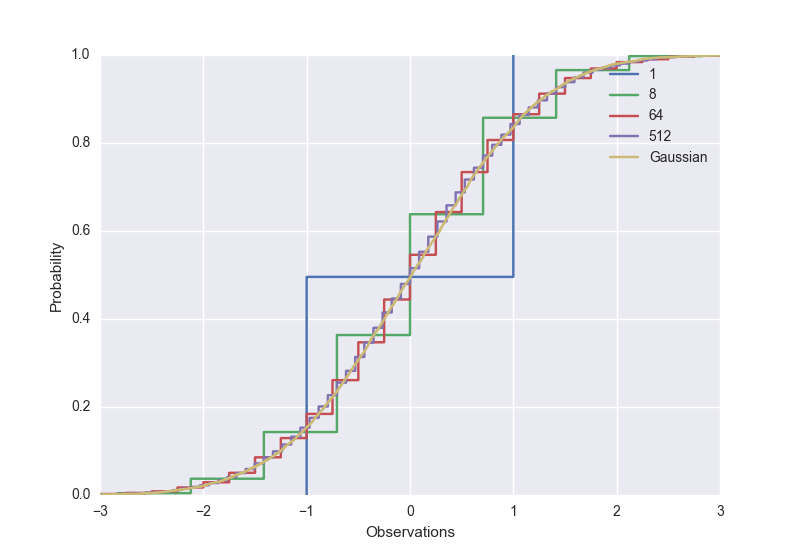
\includegraphics[width=4in]{full.png}
    \end{center}
    
    \subsubsection*{What to Submit:}
    \begin{itemize}
        \item \textbf{Part~\ref{prob:cltcdf:gaussian}:} Value for $n$ (Hint: You will need to print it)
        \item \textbf{Parts a and \ref{prob:cltcdf:k}:} In 1-2 sentences: How does empirical CDF change with $k$?
        \item \textbf{Parts~\ref{prob:cltcdf:gaussian} and~\ref{prob:cltcdf:k}:} Plot of $\widehat{F}_n(x) \in [-3, 3]$
        \item \textbf{Code} on Gradescope through coding submission
    \end{itemize}
\end{aprob}

\end{document}
